\documentclass[a4paper,12pt]{article}
\usepackage{amsmath, amsthm}
\usepackage{datetime}
\usepackage{framed}
\usepackage{enumitem}
\usepackage{fancyref}
\usepackage{wrapfig}
\usepackage{pifont}
\usepackage{appendix}

\usepackage{tikz}
\usetikzlibrary{fit,arrows,calc}

\usepackage{csquotes}
\renewcommand{\mkbegdispquote}[2]{\itshape}

\newdateformat{nianyueri}{ \THEYEAR 年 \THEMONTH 月 \THEDAY 日 }

\usepackage{xstring}
\usepackage{catchfile}
\CatchFileDef{\HEAD}{../.git/refs/heads/master}{}
\newcommand{\gitrevision}{%
  \StrLeft{\HEAD}{7}%
}

\usepackage{data/circledsteps}
\usepackage[top=1in,bottom=1in,left=1in,right=1in]{geometry} % 用于设置页面布局
\usepackage{xeCJK} % 用于使用本地字体
\usepackage[super, square, sort&compress]{natbib} % 处理参考文献
\usepackage{titlesec, titletoc} % 设置章节标题及页眉页脚
%\usepackage{xCJKnumb} % 中英文数字转换
\usepackage{amssymb}
\usepackage{amsmath} % 在公式中用\text{文本}输入中文
\usepackage{diagbox}
\usepackage{multirow} % 表格中使用多行
\usepackage{booktabs} % 表格中使用\toprule等命令
\usepackage{rotating} % 使用sidewaystable环境旋转表格
\usepackage{tabularx}
\usepackage{graphicx} % 处理图片
\usepackage{footnote} % 增强的脚注功能,可添加表格脚注
\usepackage{threeparttable} % 添加真正的表格脚注,示例见README
\usepackage{hyperref} % 添加pdf书签

\usepackage{tikz}
\usetikzlibrary{shapes,arrows,shadows}

% 字体设置
\setmainfont{Times New Roman}
\setsansfont[Scale=MatchLowercase,Mapping=tex-text]{PT Sans}
\setmonofont[Scale=MatchLowercase]{PT Mono}
\setCJKmainfont[ItalicFont={Kaiti SC}, BoldFont={Heiti SC}]{Songti SC}
\setCJKsansfont{Heiti SC}
\setCJKmonofont{Songti SC}
% \setCJKmainfont[BoldFont={FZXiaoBiaoSong-B05S}]{Songti SC}
% \setCJKfamilyfont{kai}[BoldFont=Heiti SC]{Kaiti SC}
% \setCJKfamilyfont{song}[BoldFont=Heiti SC]{Songti SC}
% \setCJKfamilyfont{hei}[BoldFont=Heiti SC]{Heiti SC}
% \setCJKfamilyfont{fsong}[BoldFont=Heiti SC]{Songti SC}
% \newcommand{\kai}[1]{{\CJKfamily{kai}#1}}
% \newcommand{\hei}[1]{{\CJKfamily{hei}#1}}
% \setromanfont[Mapping=tex-text]{TeXGyrePagella}
% \setsansfont[Scale=MatchLowercase,Mapping=tex-text]{TeXGyrePagella}
% \setmonofont[Scale=MatchLowercase]{Courier New}
%%设置常用中文字号,方便调用
\newcommand{\erhao}{\fontsize{22pt}{\baselineskip}\selectfont}
\newcommand{\xiaoerhao}{\fontsize{18pt}{\baselineskip}\selectfont}
\newcommand{\sanhao}{\fontsize{16pt}{\baselineskip}\selectfont}
\newcommand{\xiaosanhao}{\fontsize{15pt}{\baselineskip}\selectfont}
\newcommand{\sihao}{\fontsize{14pt}{\baselineskip}\selectfont}
\newcommand{\xiaosihao}{\fontsize{12pt}{\baselineskip}\selectfont}
\newcommand{\wuhao}{\fontsize{10.5pt}{\baselineskip}\selectfont}
\newcommand{\xiaowuhao}{\fontsize{9pt}{\baselineskip}\selectfont}
\newcommand{\liuhao}{\fontsize{7.5pt}{\baselineskip}\selectfont}

% 章节标题显示方式及页眉页脚设置
% \item xCJKnumb是自己额外安装的包
% \item titleformat命令定义标题的形式
% \item titlespacing定义标题距左、上、下的距离
\titleformat{\section}{\raggedright\large\bfseries}{\thesection}{1em}{}
\titleformat{\subsection}{\raggedright\normalsize\bfseries}{\thesubsection}{1em}{}
\titlespacing{\section}{0pt}{*0}{*2}
\titlespacing{\subsection}{0pt}{*0}{*1}
% 由于默认的2em缩进不够,所以我手动调整了,但是在windows下似乎2.2就差不多了,或者是article中没有这个问题
\setlength{\parindent}{2.2em}

% 设置表格标题前后间距
\setlength{\abovecaptionskip}{0pt}
\setlength{\belowcaptionskip}{0pt}


\renewcommand{\refname}{\bfseries{参~考~文~献}} %将Reference改为参考文献(用于 article)
% \renewcommand{\bibname}{参~考~文~献} %将bibiography改为参考文献(用于 book)
\renewcommand{\baselinestretch}{1.38} %设置行间距
\renewcommand{\figurename}{\small\ttfamily 图}
\renewcommand{\tablename}{\small\ttfamily 表}


\usepackage{stmaryrd}
\usepackage{mathtools}

\xeCJKsetwidth{‘’“”}{1em}

\usepackage[acronym,xindy]{glossaries}
\renewcommand*{\glossaryname}{术~语~列~表}
\makeglossaries

\usepackage[xindy]{imakeidx}
\makeindex

\loadglsentries[main]{glossary}

\title{有效过程与自然法则}
\date{1985 年 9 月 9 日}
\author{罗伯特·罗森}

\begin{document}
\maketitle{}
\centerline{\rule{13cm}{0.4pt}}

\centerline{ 苑明理 (译) }
\centerline{ 杨文波 (校) }
\centerline{ 第 \space\gitrevision\space 版}
\centerline{ \nianyueri\today }

\centerline{\rule{13cm}{0.4pt}}
\renewcommand{\contentsname}{\hfill\bfseries 目录\hfill}
\setcounter{tocdepth}{2}
\tableofcontents
\centerline{\rule{13cm}{0.4pt}}
\newpage

\section{引言}

现代科学史上最引人注目的思想交汇之一,发生在 1931 年哥德尔关于形式不可判定性原始论文发表\footnote[1]{译注:即\cite{GodelK1931}}
与 1943 年麦卡洛克和皮茨关于神经网络著作\footnote[2]{译注:McCulloch, W. and W. Pitts. “A logical calculus of the ideas immanent in nervous activity.” Bulletin of Mathematical Biology 52 (1943): 99-115.}发表之间的短短几年间。
在这十二年中,\gls{逻辑学}、数学、大脑理论和\gls{数字计算}的可能性之间建立了基本的相互关系,现在想起来所有这些仍然让人叹为观止。
人们当时认为,半个世纪之后的今天也依然认为,这些思想预示着一场根本性的革命,恰如三个世纪前牛顿所取得的进展一样。

\begin{figure}[ht]
\centering
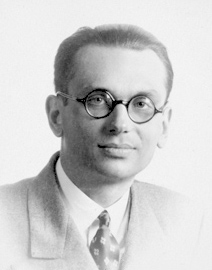
\includegraphics[height=1.5in]{images/kurt_godel.jpg}
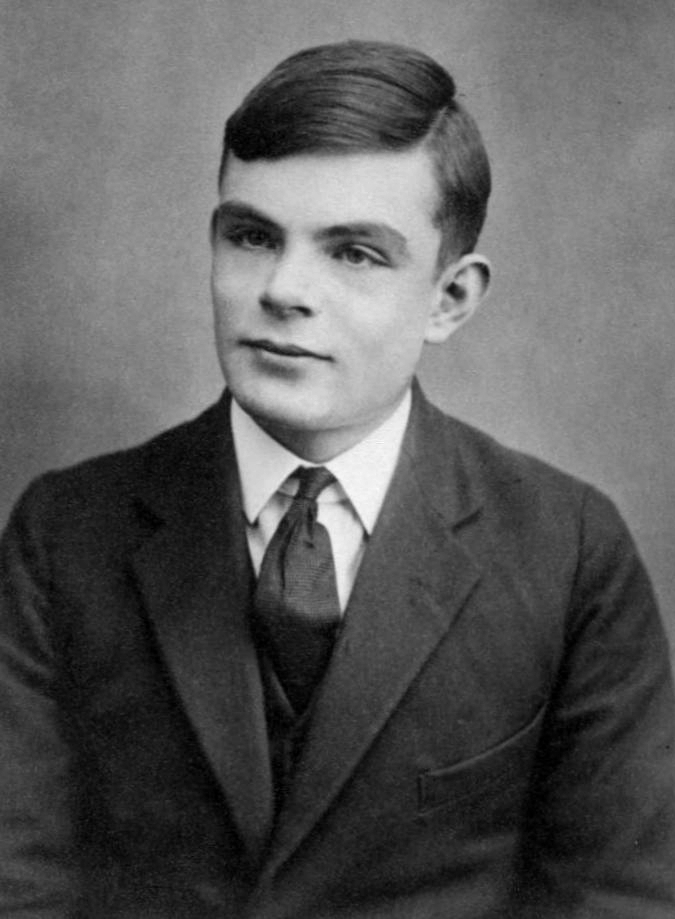
\includegraphics[height=1.5in]{images/alan_turing.jpg}
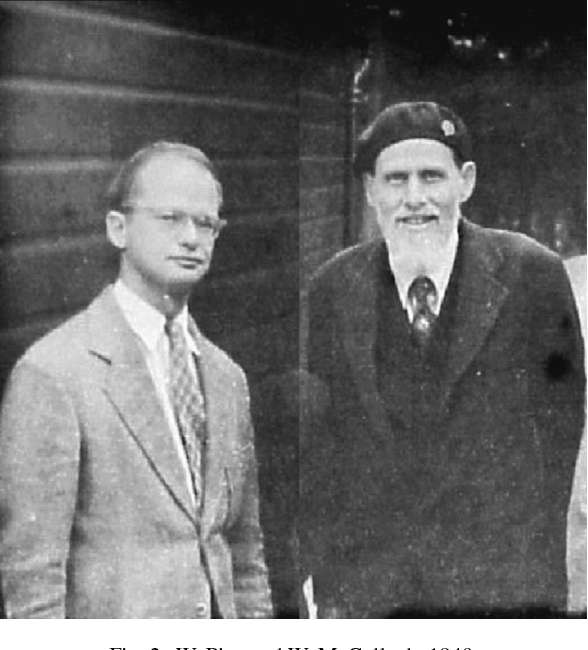
\includegraphics[height=1.5in]{images/pitts_mcculloch_1949.png}
\caption{青年哥德尔;青年图灵;皮茨和麦卡洛克的合照}
\end{figure}

阿兰·图灵的名字在这些惊人发展的历史上是非同寻常的。正是因为图灵,在他 1936 年发表的开创性论文\footnote[3]{译注:即\cite{TuringA1937}}中,通过构建以他名字命名的“机器”类,首次把这些相关的思想真正并列在一起。
首先,\textbf{\gls{图灵机}}是从人类进行数学计算的心理过程中明确推演出来的;其次,它们代表了一种逻辑或算法过程的\gls{形式化}体现,如同它们在数学中的表现一样;
再者,通过使用“机”这个术语,它们又代表了,利用\gls{物质过程}来扩展我们自己的数学能力(很快会通过\gls{数字计算机}的发明来实现),并且在更深的层次上,为探索生命本身建立一个新的、强大的隐喻。

\begin{figure}[ht]
\centering
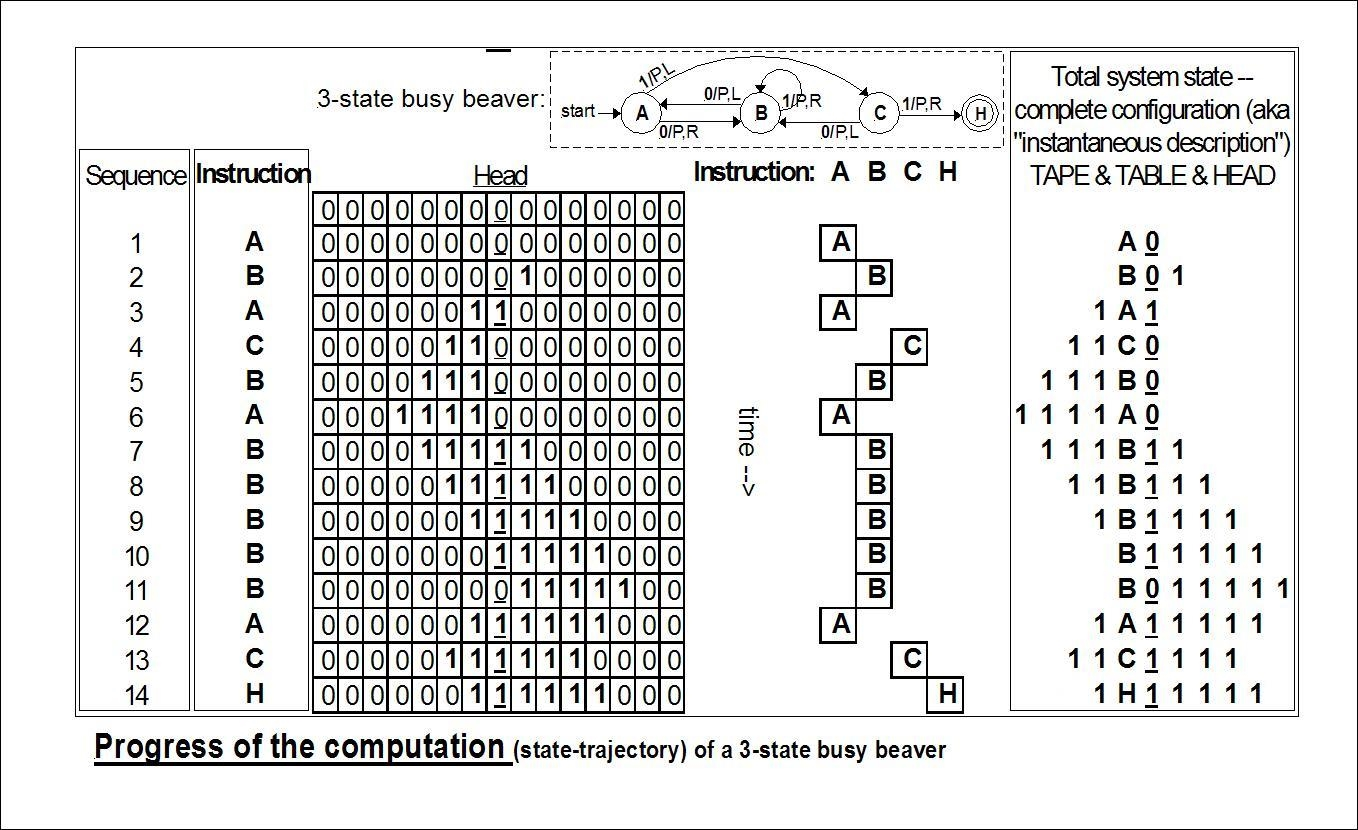
\includegraphics[height=2.0in]{images/turing_machine.jpg}
\caption{计算忙碌海狸问题的图灵机}
\end{figure}

在纯粹的数学/逻辑的层面上,人们很快认识到,\gls{图灵机}是体现\textbf{\gls{算法}}概念的许多等价形式之一。依次来说,\gls{算法}被认为是一个解决问题的\textbf{\gls{有效过程}}的缩影。
然后,一个\gls{有效过程}意味着一种绝对必要性;它是一个\gls{推理链条},对于从适当初始数据开始的每一个情况,它都\textbf{必须}要导向相应的那个答案或解答。
更进一步,\gls{算法}是一个\textbf{死记硬背}的过程,一旦启动,在从数据到解答的无休止的过程中,不需要进一步的干预、省察和思考。这就是为什么,现在回想起来,
把它体现在一台“机器”上是如此自然,就像图灵做的那样。

\begin{wrapfigure}{r}{0.25\textwidth}
  \begin{center}
    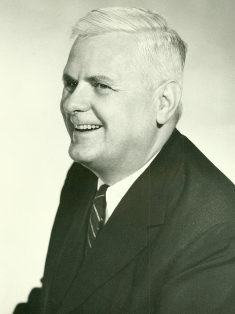
\includegraphics[height=2.0in]{images/alonzo_church.jpg}
  \end{center}
  \caption{阿隆佐·邱奇}
\end{wrapfigure}

由于“\gls{有效过程}”的提法是一个非形式的、直观的概念,而“\gls{算法}”的提法是一个精确的\gls{形式化}的数学概念,很早就有人提出后者可以取代前者。
这正是\textbf{\gls{邱奇论题}}的实质内容\cite{KleeneSC1952},该论题断言,任何人们想称之为“有效”的过程,都已可以通过一些适当编程的\gls{图灵机}来完成。

现在,严格地说,到目前为止所描述的所有讨论都是完全\gls{形式化}的;它们发生在\gls{命题}和\gls{产生规则}的逻辑和数学宇宙中。从某种意义上说,它们都是“\gls{软件}”。
然而,有趣之处主要集中在这样一个事实:像“机器”或“有效”这样的术语具有非数学的内涵,这些内涵都从属于自然\gls{物质现象}的外部世界。
事实上,正如我们已经注意到的,图灵自己设计的数学机器是从现实世界的现象中抽象得来的,一个人在进行计算。
这种暗示如此不可抗拒地传达出, 如果人类精神活动的\textbf{这一}方面可以“机械化”,为什么其他方面不可以呢? 为什么不可以全部呢?
同样地,如果心理过程,包括在物质大脑中发生的事情(也即在\gls{硬件}中)可以完全形式地表示,
为什么不能有其他类型的\gls{物质系统}(也即其他\gls{硬件})可以做与大脑相同的事情?
虽然还在胚胎阶段,在这里,我们看到了,“\gls{人工智能}”最广的推论,和许多其他的意涵。

但是,一旦我们承认“机器”或“有效”这样的词具有\gls{物质}意义,我们就离开了数学的世界,进入了(最广义的)物理世界。正如我们已经提到的,\gls{图灵机}是“纯软件”的,
而物理学则相反,是“纯\gls{硬件}”的。因此,无论是好是坏,我们引入了\gls{硬件}和\gls{软件}之间的根本区别,它本身并不是我们开始时所使用的\gls{形式理论}的一部分;同样,它也不是物理学的一部分。
正如我们将要看到的,这种区别是至关重要的,但是也是隐蔽的,藏在包罗万象的总称“机器”中。从马丁·戴维斯的《可计算性和不可解性》\cite{DavisM1958}一书中,
我们可以看到这种区别是如何悄无声息地出现的:

\begin{displayquote}
    我们怎么能排除某一天(也许是某个外星访客)给我们一个(也许是极其复杂的)设备或“\gls{神谕}”来“计算”一个\gls{不可计算}函数的可能性呢?
\end{displayquote}

这显然是在一个完全\gls{形式化}的数学进展背景下提出的最具修辞性的反问句。但是我们在这里清楚地看到术语“机器”的模糊性\footnote[1]{译注:?},
它建立在真实\gls{硬件}和逻辑\gls{软件}之间的默认区别之上。

\begin{figure}[ht]
\centering
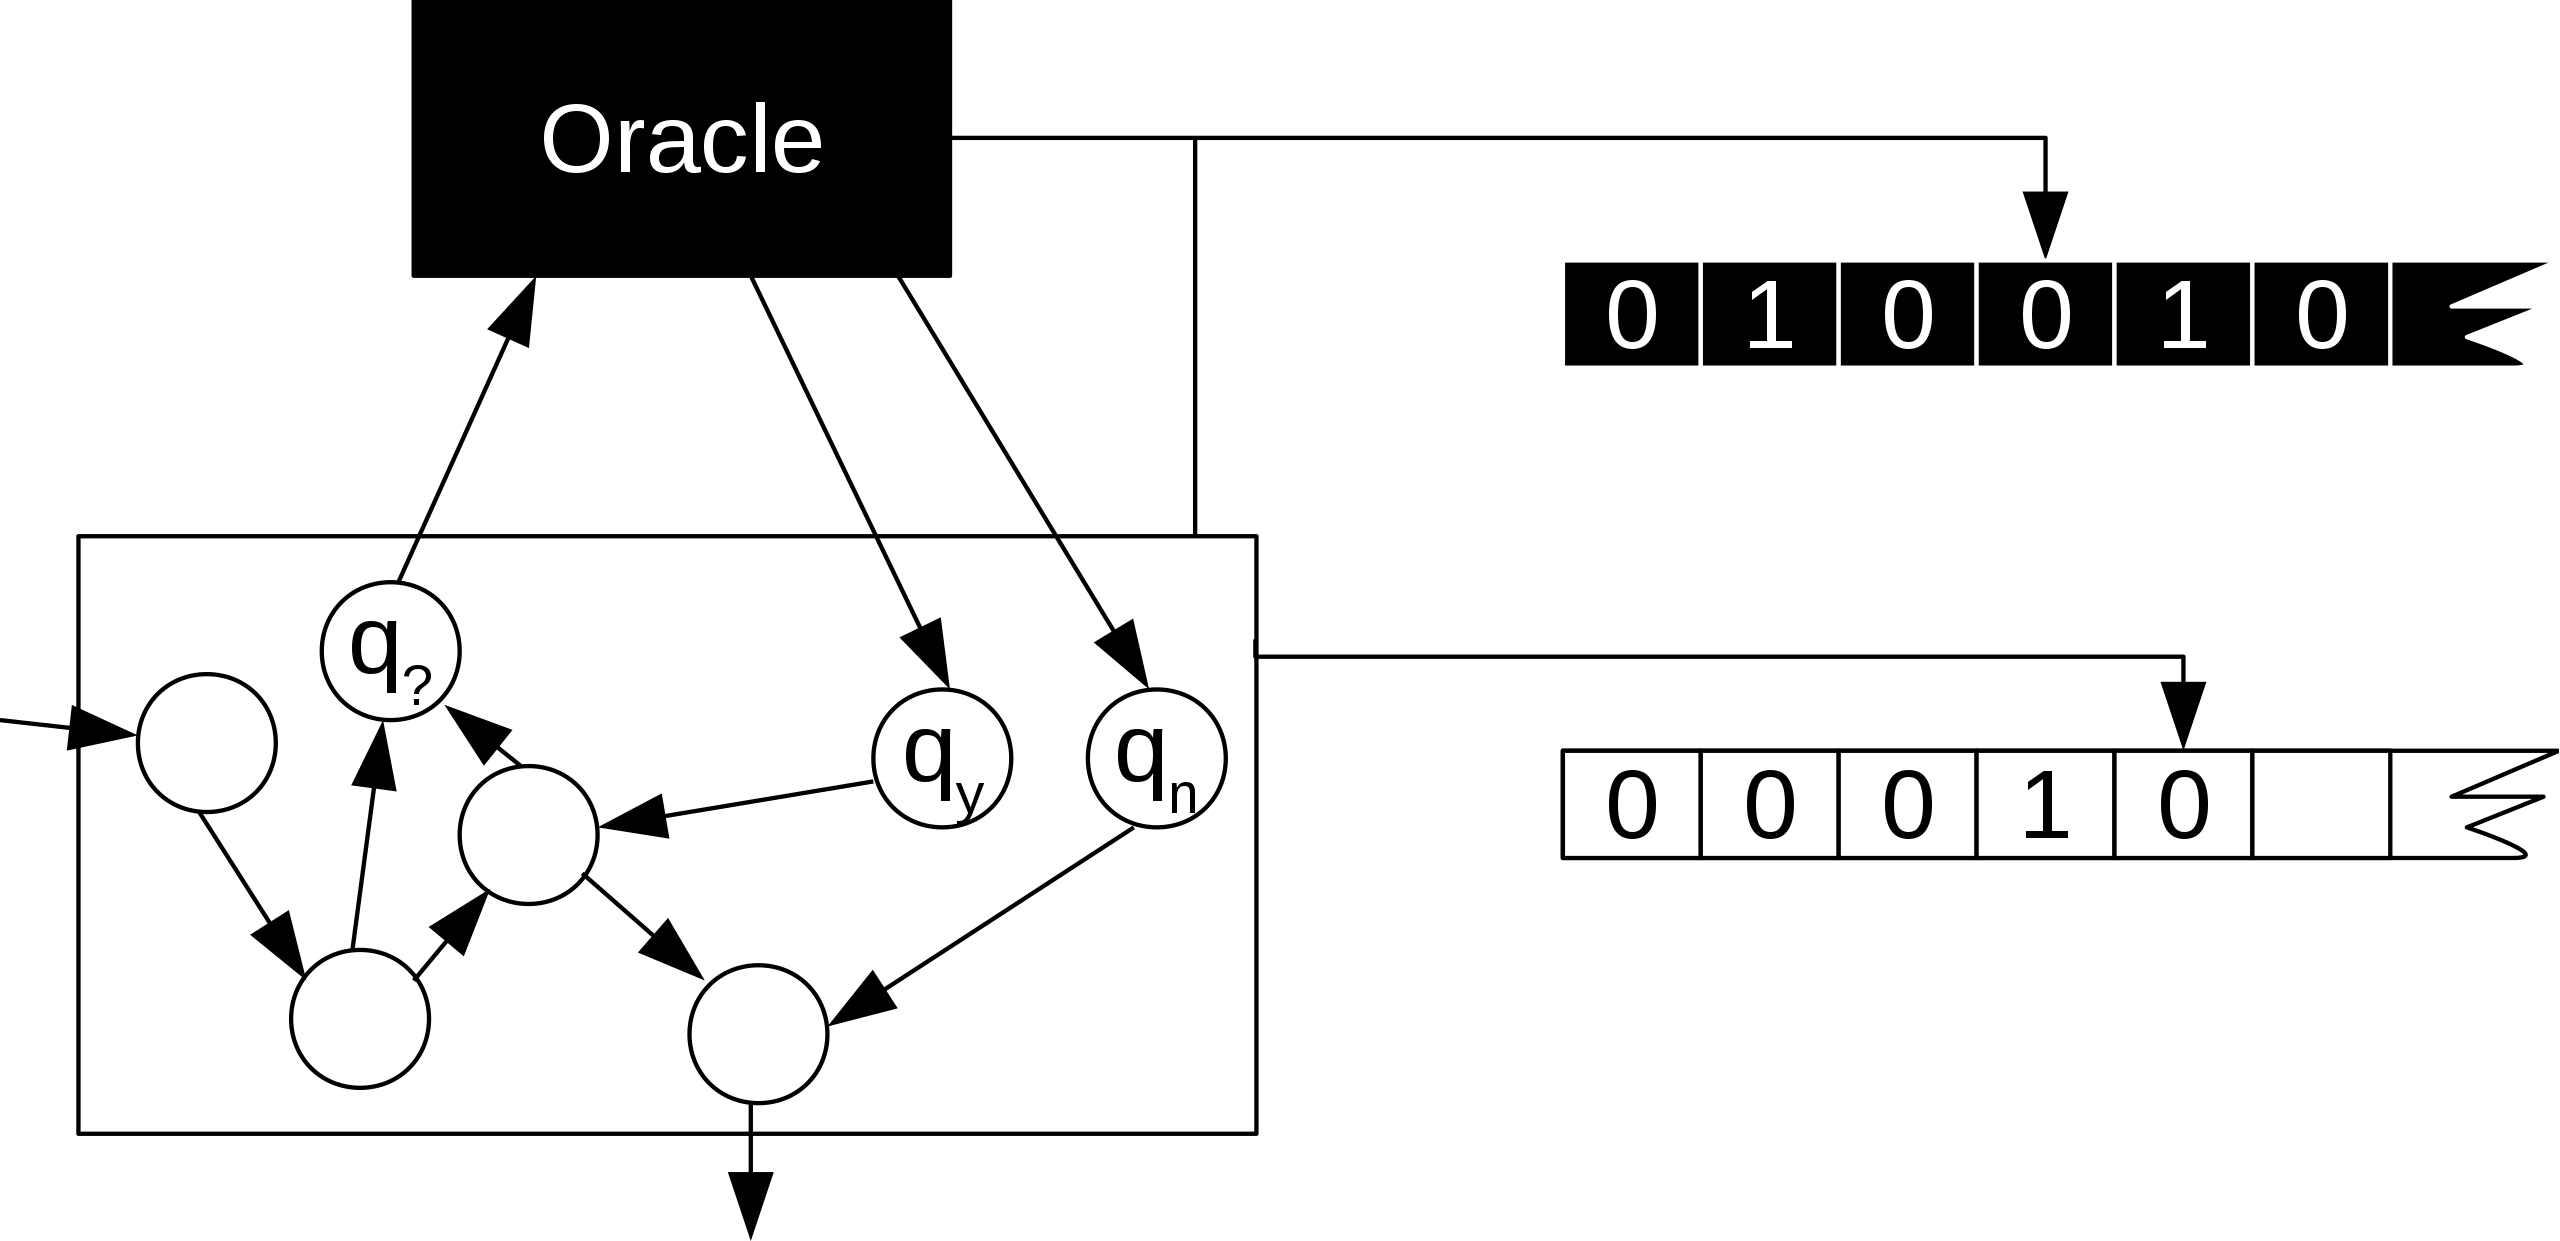
\includegraphics[height=2.0in]{images/turing_machine_oracle.png}
\caption{神谕图灵机}
\end{figure}

长期以来,作者一直为这一问题的深层认识论的推论所困扰\cite{RosenR1962}。尤其是,一旦我们承认“\gls{硬件}”或\gls{物质系统}进入我们的讨论
(正如我们已经指出的那样,这从一开始就是明确无误的意图), 那么“\gls{有效过程}”的概念会发生什么变化呢?
很久以前\cite{RosenR1962},我考虑过\gls{邱奇论题}在这个新的背景下意味着什么? 特别是:
邱奇论题是否是对\gls{物质}本性的一个基本限制呢(类似于热力学定律排除了\textbf{永动机})?
抑或是相反?如果邱奇论题可以被自然过程破坏,那么递归性又会怎么样呢?

在这里回顾一下先前论点的要点可能是有用的。假设我们有一个\textbf{物理}系统 $S$(也许是戴维斯的外星“计算机”)。它的行为受到物理定律的支配,我们通过实验来了解这些定律。
一个典型的实验要么对系统做一些事情(例如,从外部扰动它),要么让系统对其环境做一些事情,然后\gls{观察}或\gls{测量}结果。显然,实验者的\gls{干预}和\gls{测量}的结果都是\gls{物质事件}。
\gls{事件}是由数字来描述或刻画其特性的,其数值是由应用的合适的量表来决定的\cite{RosenR1978}。为了简单起见,假设我们的实验干预 $\alpha$ 拥有的属性是这样一个数值 $r(\alpha)$,
而我们系统的结果行为由另一个这样的数字刻画。通过这种方式,我们的实验者可以生成一个数值表,它定义了\textbf{一个从数字到数字的函数}  \begin{equation}\label{eq:1} f: r(\alpha) \mapsto \beta\end{equation}

读者将会认识到,这个过程以典型输入输出的方式刻画了我们系统 $S$。函数 $f$ 的形式,清楚地告诉我们支配 $S$ 行为的\textbf{规律}。毕竟,这就是\gls{科学实验}的全部功用。

这个实验过程在某种意义上是有效的。事实上,正如我们将在下面详细论述的那样,\gls{物质世界}(例如,在系统 $S$ 中)的\gls{事件序列}是由\textbf{\gls{因果关系}}所支配的,这些因果关系将它们联系在一起,就像\gls{蕴涵关系}将\gls{命题}无可避免地联系在一起一样。
因此,如果我们的实验过程是\textbf{\gls{可复现}}的(这意味着 $S$ 中相同的\gls{因果序列}可以随意重建),那么\gls{邱奇论题}必须意味着\textbf{任何输入输出函数\hyperref[eq:1]{$f$},从我们已经描述过的任何\gls{物质系统} $S$ 中\gls{生成},它必须是递归的或\gls{可计算}的}。
否则,系统 $S$ 将正是戴维斯向我们保证排除在可能性之外的那种“计算机”。

从这个角度来看,\gls{邱奇论题}试图从\gls{软件}(\gls{算法})的前提中得出关于\gls{硬件}(物理学)的推论或结论。
冯·诺依曼关于“自我复制”的论点\cite{BurksA1966}体现了另一种众所周知的同样尝试。
在这里,我们的目的是从一个关于计算的\textbf{\gls{形式}}理论中学习关于\textbf{\gls{物质}}系统(特别是有机体)的行为的一些东西。
不出所料,这类尝试风险极大,但\textbf{如果}能成功实现,回报将是巨大的。

\begin{figure}[ht]
\centering
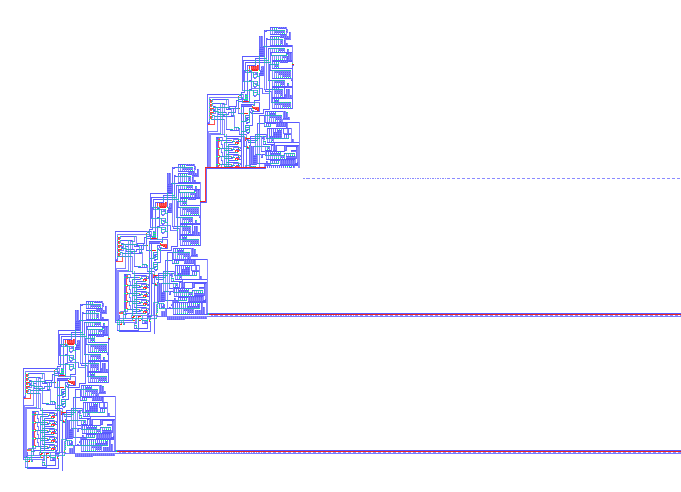
\includegraphics[height=2.0in]{images/self_reprod.png}
\caption{运行中的第一个为人所知的自复制机}
\end{figure}

至少,我们可能已经看到,在\gls{形式理论}中引入“\gls{硬件}”的概念将产生一些特殊的结论。而当我们试图把“\gls{软件}”的概念引入物理学时,互补的结论就出现在另一方面。
然而,这些特殊的结论将告诉我们一些关于这两者的有趣事情。在本文的其余部分,我们将探索这种可能性。

\section{形式系统中的邱奇论题}

\gls{邱奇论题}的实质是,把任何\gls{形式系统}中的\textbf{\gls{逻辑推理}}与\textbf{\gls{字符串处理}}等同起来。然后,\gls{字符串处理}或字处理是一种纯粹的\textbf{\gls{语法}}活动。
\gls{字符串处理},当然,正是\gls{图灵机}所做的。尽管如此,从表面上看,这似乎是一个非常强的、或许有些过于强的条件,
它要求\gls{形式系统}中的每一个\gls{推理},都应该\textbf{只}用\gls{语法项}来表达;也就是说,从前提到结论的每一个步骤,都应该完全通过,对这些\gls{编码}了的\gls{命题}的符号进行操作来实现。

然而,我们可以有一个相当有力的理由来支持这个看起来不太可能的论题。
它源自于一种\gls{形式化}的趋势,这种趋势始于欧几里德,随着非欧几何的发现(作为\gls{形式系统},和上帝赋予的欧氏几何一样,是一致的几何学),
以及发现朴素集合论中悖论时的绝对绝望,这种混乱成为了一个紧迫问题。
大卫·希尔伯特开创的\gls{形式主义}对这种情况的回应,恰恰是要清空数学的任何\gls{语义内容},辩称这些不必要的\gls{语义},是困难的根源。
实际上,这把所有的数学变成了一种游戏,在这种游戏中,无意义的符号按照(一种有限的)任意\gls{语法规则}来处理。
事实上,希尔伯特\gls{形式主义}的全部意义,在于创造一个除了\gls{语法}以外什么都没有的系统。

\begin{figure}[ht]
\centering
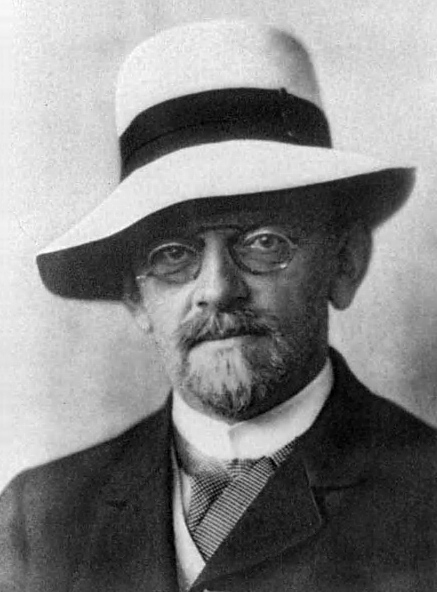
\includegraphics[height=2.0in]{images/hilbert.jpg}
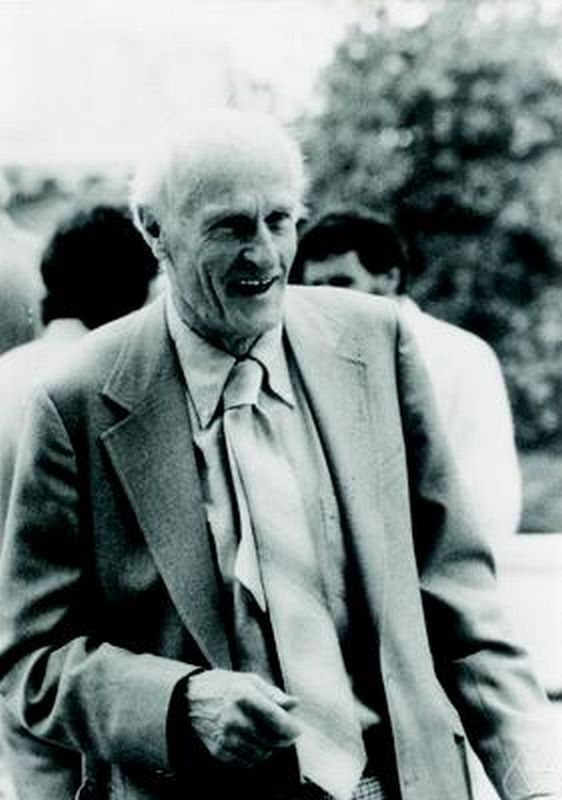
\includegraphics[height=2.0in]{images/kleene.jpg}
\caption{大卫·希尔伯特;斯蒂芬·科尔·克莱尼}
\end{figure}

或许,这种\gls{形式主义}计划最清晰的陈述是由克莱尼给出的\cite{KleeneSC1952}

\begin{displayquote}
这一步(\gls{公理化})将不会完成,直到所有的未定义的性质或理论的技术性术语已表示成\gls{公理},它们对\gls{定理}的推演是重要的。
然后应该有可能应用演绎法,把技术术语当作没有意义的单词。
因为,说它们对于\gls{定理}的推导具有必要的意义,而不是说它们是从支配的\gls{公理}中衍生出来的,
就等于是说,对于定理演绎至关重要的属性还未完全表达为\gls{公理}。
当技术性术语的含义因此被忽略了,我们就达到了形式公理学说的立场……
因为我们已经完全从内容中抽象出来,只留下\gls{形式},我们说原始理论已经\gls{形式化}了。
在这种结构中,理论不再是一个有意义的命题系统,而是一个作为词序列的句子系统,这些词序列依次是字母序列。
我们只是参照\gls{形式}来说,哪些单词组合成句子,哪些句子是\gls{公理},哪些句子是其他句子的直接后果。
\end{displayquote}

显然,这里的想法是,总是可以用\gls{语法}替换\textbf{\gls{语义}}(“意义”),从而在\textbf{\gls{逻辑}}上没有信息丢失;
任何涉及\gls{语义}的\gls{推理},在\gls{形式化}中都有纯粹的\gls{语法}映像。

在这样的一个\gls{形式系统}中,我们首先认为\gls{公理}是\textbf{真}的。这种真的概念是\textbf{可传递}的;
如果\gls{公理}为真,那么通过将系统的\gls{推理规则}应用于它们而获得的符号序列也是如此;因而,真从\gls{公理}传递到\gls{定理}。
到目前为止,我们从来不需要从外部引入“真”的概念到系统中,就像从前一样;我们只是在推演的过程中构造真的\gls{命题}(\gls{定理})。

\begin{figure}[ht]
\centering
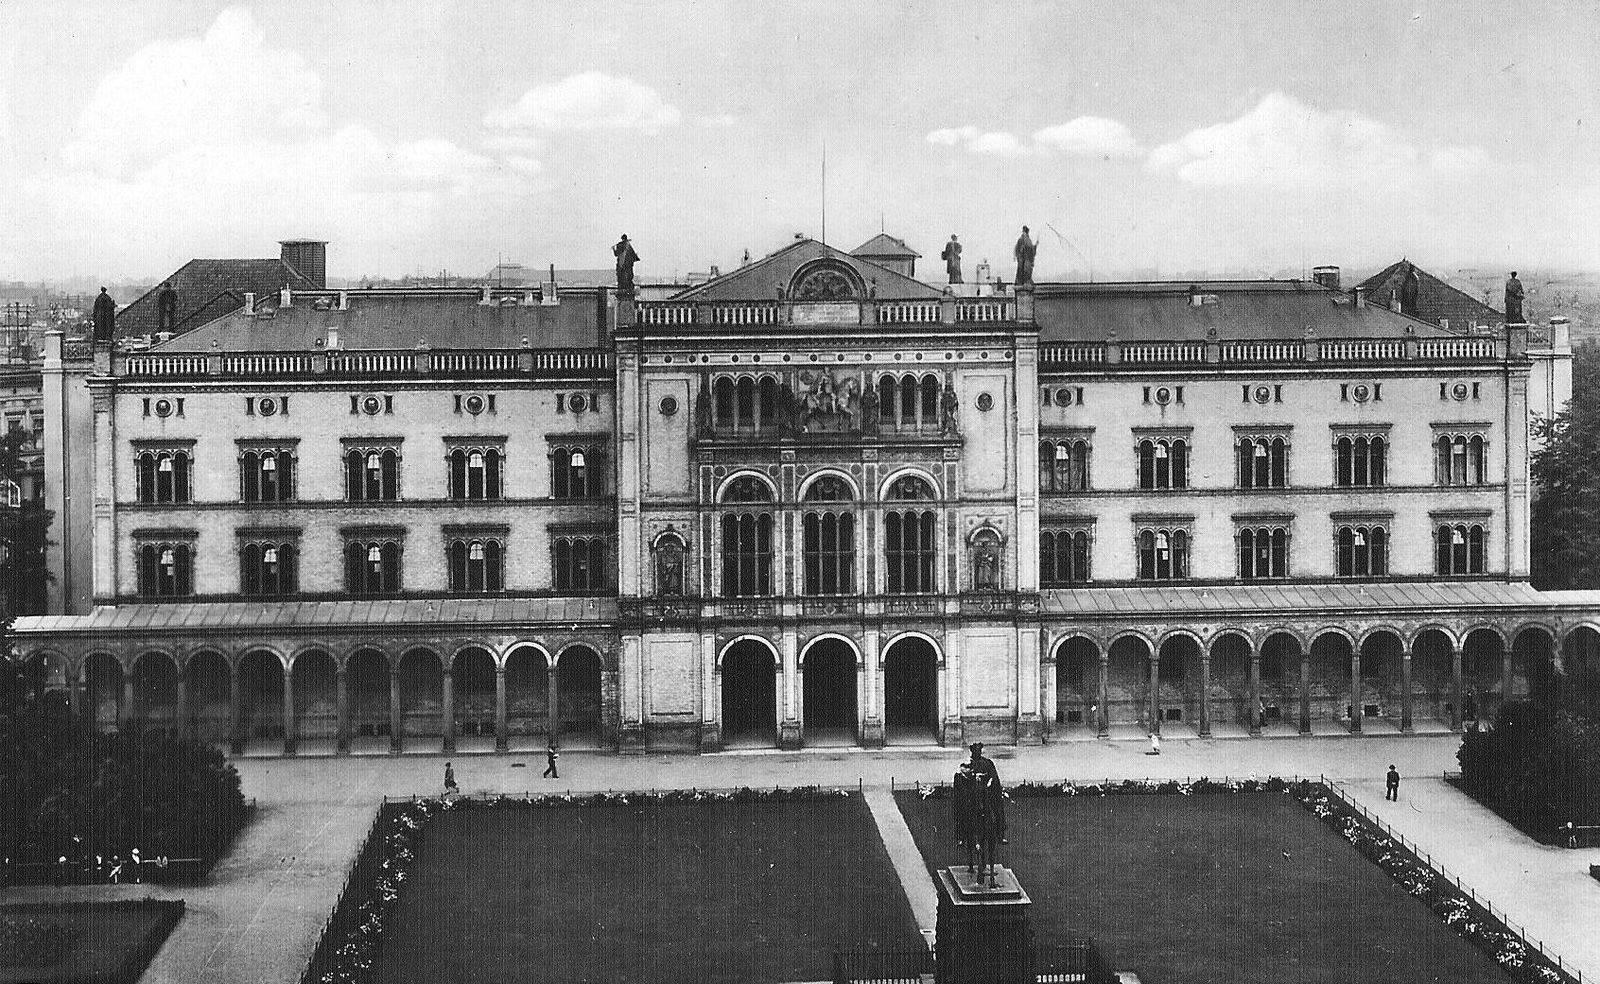
\includegraphics[height=2.5in]{images/konigsberger_university.jpg}
\caption{哥德尔不完备性定理最早于 1930 年 9 月在柯尼斯堡大学的一个学术会议上发表}
\end{figure}

哥德尔著名的定理\cite{GodelK1931}中所包含的麻烦,源自于试图将这种\textbf{内部}真理的构造性概念与\gls{形式算术}中预先赋予的\textbf{外部}真值进行比较;正如哥德尔所示,它们并不匹配。
此外,看待图灵可判定性定理\cite{TuringA1937}的一种方式是,在给定的\gls{形式化}中,\textbf{没有内部\gls{推理机制}}来决定一个\gls{命题}是否是一个\gls{定理}(即,是真的)。

因此,我们\textbf{知道},\gls{形式主义}计划,其中只有纯粹的\gls{语法}推论是允许的,是过于贫乏的,甚至不足以支撑数论。
也就是说,我们要么允许一些“非形式”的\gls{推理过程}进入我们的系统,根据哥德尔定理,这些过程甚至在原则上都\textbf{不能}简化为\gls{语法}; 要么永远把我们自己限制在数论的片段中。
这种“非形式”的\gls{推理过程}是\gls{邱奇论题}所不允许的,它们是\textbf{无效的}。

让我们用更熟悉的术语来讨论上述问题。 在普通(“柏拉图式”)数学中,它同时具有\gls{语法}和\gls{语义}的方面,
我们知道,如果我们给定一个集合 $S$ ,通过规范结构可以从 $S$ 构造出许多其他集合。
例如,我们有幂集 $2^S$ ,我们有 $S$ \gls{生成}的自由代数结构(半群,群等) ,我们有从 $S$ 到 $S$ 的所有映射的集合 $H(S, S)$ ,
我们有笛卡儿积 $S \times S$ ,等等。
这些相关的集合赋予我们\textbf{\gls{推理能力}},这些能力具有\gls{逻辑关系}的力量,但这些支配 $S$ 的数学系统的形式推演律,并不必然有足够的表达力。
例如,如果 $Q: S \mapsto S$ 是一个自同构(即 $H(S, S)$ 的一个元素) ,对 $s \in S $,我们可以说 $Q(s) = s^{\prime}$ 在 $s$ 和 $s^{\prime}$ 之间建立了一个\gls{蕴涵关系}。
但是,这种“\gls{蕴涵}”不一定与我们可以从支配系统的产生式规则中得出的结论相一致,也就是说,不必仅仅遵循系统的\gls{语法}。
如果两者是一致的,可以说我们的 $Q$ 在系统中是\textbf{\gls{可计算}}的;否则,就不是\textbf{可计算}的。在后一种情况下,根据\gls{邱奇论题},我们不得不说映射 $Q$ 不是\textbf{有效}的。
但是很明显,如果 $Q$ 有意义或存在,一旦它被赋予给我们,它就\textbf{是}有效的。

在\gls{形式系统}的“全\gls{软件}”的世界中,我们当然可以用任何喜欢的方式来限定自己。
因此,我们可以不允许我们自己拥有任何无法表示成纯粹\gls{语法项}的自同构 $Q$。
在这样一个世界里,也只有在这样一个世界里,\gls{邱奇论题}才能不受限制地成立。
当然,这样的一个\gls{形式化}的世界到底是否有趣,是另一个问题。正如我们将看到的,当我们允许“\gls{硬件}”进入我们的世界时,情况会变得更加糟糕。

在讨论\gls{物质系统}之前,我们略谈下编解码,即把\gls{形式系统}中的\gls{命题}\gls{编码}到\gls{图灵机}的码带上,以及把码带上的内容\gls{解码}成系统中的\gls{命题}。
很明显,在\gls{编码}和\gls{解码}方面,我们可以按照通常的直观意义使用“有效”一词;例如,我们熟悉的\gls{哥德尔编码},
显然是从\gls{语法}到算术、然后再回来的有效映射。事实上,为了表明一个过程在某些\gls{形式系统}中是有效的,或者说是递归的,
我们可以清楚地将\gls{编码}、计算和\gls{解码}结合到一个单独的\gls{图灵机}中,这个机器可以完成所有三个步骤。
然而,我们在这里只是记下,\gls{编码}和\gls{解码}在\gls{逻辑}上彼此不同,也不同于实际计算;
如果它们在某种意义上是“无效”的,那么\gls{邱奇论题}可能会失败,即使计算本身是完全递归的。

\section{蕴涵与因果}

正如我们已经看到的,在\gls{形式系统}的领域,\gls{邱奇论题}辨析了“\gls{有效过程}”的直觉概念与纯粹的\gls{语法}观点下的\gls{字符串处理}。

\begin{figure}[ht]
\centering
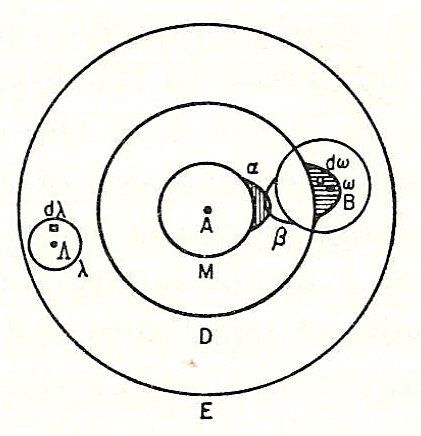
\includegraphics[height=2.5in]{images/boltzmanns_molecule.jpg}
\caption{玻尔兹曼设想的由原子构成的分子}
\end{figure}

也就是说,任何可以在系统内“有效地”执行的\gls{蕴涵},都可以通过一套有限的产生规则来执行,这套规则操作于从一个有限字母表中取出的有限的符号串。

我们还指出,当我们在处理\textbf{\gls{物质}}世界时(相对于形式的数学和\gls{逻辑}),\gls{蕴涵}的观念被\gls{因果}的观念所取代。
尽管如此,我们仍然可以保留“有效”过程的想法。 在这种情况下,\gls{邱奇论题}意味着任何\textbf{\gls{因果序列}}都可以用相应的递归过程来表示;
也就是说,\textbf{任何\gls{因果序列}都可以用纯粹的\gls{语法}手段来描述}。 如果这是真的,它当然会严重限制\textbf{物理学}的发展。
\textbf{是否\gls{自然法则}本身可以表达成纯粹的\gls{语法项},或者它们是否可以拥有一个内在的\gls{语义}的组成部分不能被有限\gls{形式化},问题绝不仅仅限于此。}

值得注意的是,数学中的\gls{形式化}(即纯粹的\gls{语法})与理论科学中的类似趋势是完全平行的。
事实上,原子论(或者现在的“基本粒子”理论)的全部推动力是将所有\gls{物质过程}简化到终极组成单元的运动,而没有任何内部结构(“意义”),
只拥有瞬时位置(“构型”)和位置的时域导数。推动这些终极单元的力量是\gls{形式系统}中的产生式规则的精确类比。

因此,一个\gls{物质系统}在给定力的影响下所追踪到的路径或轨迹是形式\gls{定理}的类比,以初始条件为\gls{公理}。

\gls{物质系统}中\gls{事件}之间的\gls{因果关系}可以与描述这些事件的\gls{命题}之间的\gls{蕴涵关系}相联系的观点是理论科学的\textbf{必要条件}。
事实上,过去被称为\textbf{\gls{自然法则}}的信念要求:
\begin{enumerate}[label=(\alph*)]
\item 我们在外部世界中感知到的\gls{事件序列}不是任意的或异想天开的,而是受到明确规则的支配(这就是\textbf{\gls{因果关系}});
\item 这些规则可以清楚地表达出来,以便人类头脑能够理解。
\end{enumerate}
综上所述,\gls{自然法则}的这种表述精确地断言,\gls{物质系统}中的\gls{因果关系}可以被引导到一个\gls{形式化}的(终极的,数学的)命题形式系统的一致性\gls{蕴涵关系}中。

这种情况可以最简洁地用图式一来表示(参见图9)。

\begin{figure}[ht]
\centering
\begin{tikzpicture}
[round/.style={rounded corners=1.5mm, minimum width=1cm, inner sep=2mm, above right, draw, align=center, text width=7mm}]
    \node[round] (N) at (0,0) {自然系统};
    \node[round] (F) at (6,0) {形式系统};
    \path[draw, thick, bend left=-45]
        ($(N.east)+(0,-1.0)$) edge[->] node[near start] {\hspace{+6em}\ding{193}编码} ($(F.west)+(0,-1.0)$);
    \path[draw, thick, bend left=-45]
        ($(F.west)+(0,1.0)$) edge[->] node[near start] {\hspace{-6em}\ding{195}解码} ($(N.east)+(0,1.0)$);
    \path[draw, thick, bend left=-45]
        ($(N.west)+(0,+0.8)$) edge[->] node {\hspace{-3em}\ding{192}因果} ($(N.west)+(0,-0.8)$);
    \path[draw, thick, bend left=-45]
        ($(F.east)+(0,-0.8)$) edge[->] node {\hspace{+3em}\ding{194}蕴涵} ($(F.east)+(0,+0.8)$);
\end{tikzpicture}
\caption{图式一}
\end{figure}

我们说,当以下的交换性成立时,图表左侧的自然系统和右侧的\gls{形式系统}之间存在一种\textbf{\gls{建模关系}}:\begin{equation} \Circled{1} = \Circled{2} + \Circled{3} + \Circled{4}\end{equation}

也就是说,无论我们是仅仅作为\gls{观察者}坐在那里,\gls{观察}自然系统中\gls{事件}的展开序列,还是我们
\begin{enumerate}[label=(\alph*)]
\item 将自然系统的某些性质\gls{编码}到\gls{形式体系};
\item 然后利用\gls{形式系统}的\gls{蕴涵结构}导出\gls{定理};
\item 再将这些\gls{定理}\gls{解码}成关于自然系统本身的\gls{命题}(\textbf{\gls{预测}})
\end{enumerate}
我们都得到了同样的答案。当图表交换时,我们在自然系统的\gls{因果}特征和\gls{形式系统}的\gls{蕴涵结构}之间建立了一个一致性。
我们可以说\gls{形式系统}是自然系统的\textbf{\gls{模型}},或者说,自然系统是\gls{形式系统}的\textbf{实现}。

这些小图表本身包含许多丰富而重要的认识论属性,我们不能在这里进入;要进行更全面的讨论,请参阅\cite{RosenR1985}。

一旦我们建立了一个形式的系统,作为某种自然过程的\gls{模型},我们就离开了科学的领域,进入了数学的领域。
然后,我们可以像对待其他任何\gls{形式系统}一样对待\gls{模型}。特别是,我们可以看看它纯粹的\gls{语法}方面,
我们可以立即辨认出\gls{邱奇论题}里的“有效”过程,并问这些过程是否耗尽了系统本身的\gls{蕴涵性资源}。

通过这种方式,我们可以构建一个纯\gls{语法}的原本的自然系统的“机器”\gls{模型},如 图10 所示。

\begin{figure}[ht]
\centering
\begin{tikzpicture}
[round/.style={rounded corners=1.5mm, minimum width=1cm, inner sep=2mm, above right, draw, align=center, text width=7mm}]
    \node[round] (N) at (0,0) {自然系统};
    \node[round] (F) at (4,0) {形式系统};
    \node[round] (M) at (8,0) {机  器};
    \path[draw, thick, bend left=-45]
        ($(N.east)+(0,-1.0)$) edge[->] node[near start] {} ($(F.west)+(0,-1.0)$);
    \path[draw, thick, bend left=-45]
        ($(F.west)+(0,1.0)$) edge[->] node[near start] {} ($(N.east)+(0,1.0)$);
    \path[draw, thick, bend left=-45]
        ($(F.east)+(0,-1.0)$) edge[->] node[near start] {} ($(M.west)+(0,-1.0)$);
    \path[draw, thick, bend left=-45]
        ($(M.west)+(0,1.0)$) edge[->] node[near start] {} ($(F.east)+(0,1.0)$);
    \path[draw, thick, dotted, color=lightgray, bend left=-45]
        ($(N.south)$) edge[->] node[near start] {} ($(M.south)$);
    \path[draw, thick, dotted, color=lightgray, bend left=-45]
        ($(M.north)$) edge[->] node[near start] {} ($(N.north)$);
    \path[draw, thick, bend left=-45]
        ($(N.west)+(0,+0.8)$) edge[->] node {\hspace{-3em}因果} ($(N.west)+(0,-0.8)$);
    \path[draw, thick, bend left=-45]
        ($(F.east)+(0,-0.8)$) edge[->] node {\hspace{+3em}蕴涵} ($(F.east)+(0,+0.8)$);
    \path[draw, thick, bend left=-45]
        ($(M.east)+(0,-0.8)$) edge[->] node {\hspace{+5em}字串处理} ($(M.east)+(0,+0.8)$);
\end{tikzpicture}
\caption{图式二}
\end{figure}


我们只看外侧的两个系统,忘记原本的\gls{模型},这个\gls{模型}现在在两者间扮演一种“\gls{转换器}”的角色。

但是,当我们这样做时,必须明确注意以下几点:
\begin{enumerate}[label=(\alph*)]
\item 它们之间的\textbf{\gls{编码}}和\textbf{\gls{解码}}箭头(图式二中的虚线箭头)在任何形式意义上都不能被描述为\textbf{有效}的;
\item 这些\gls{编码}和\gls{解码}箭头只涉及居最右的边框中的机器的\textbf{输入}和\textbf{输出}字符串;
\end{enumerate}
这两个观察结果都很重要。我们将依次简要地讨论它们。

\begin{figure}[ht]
\centering
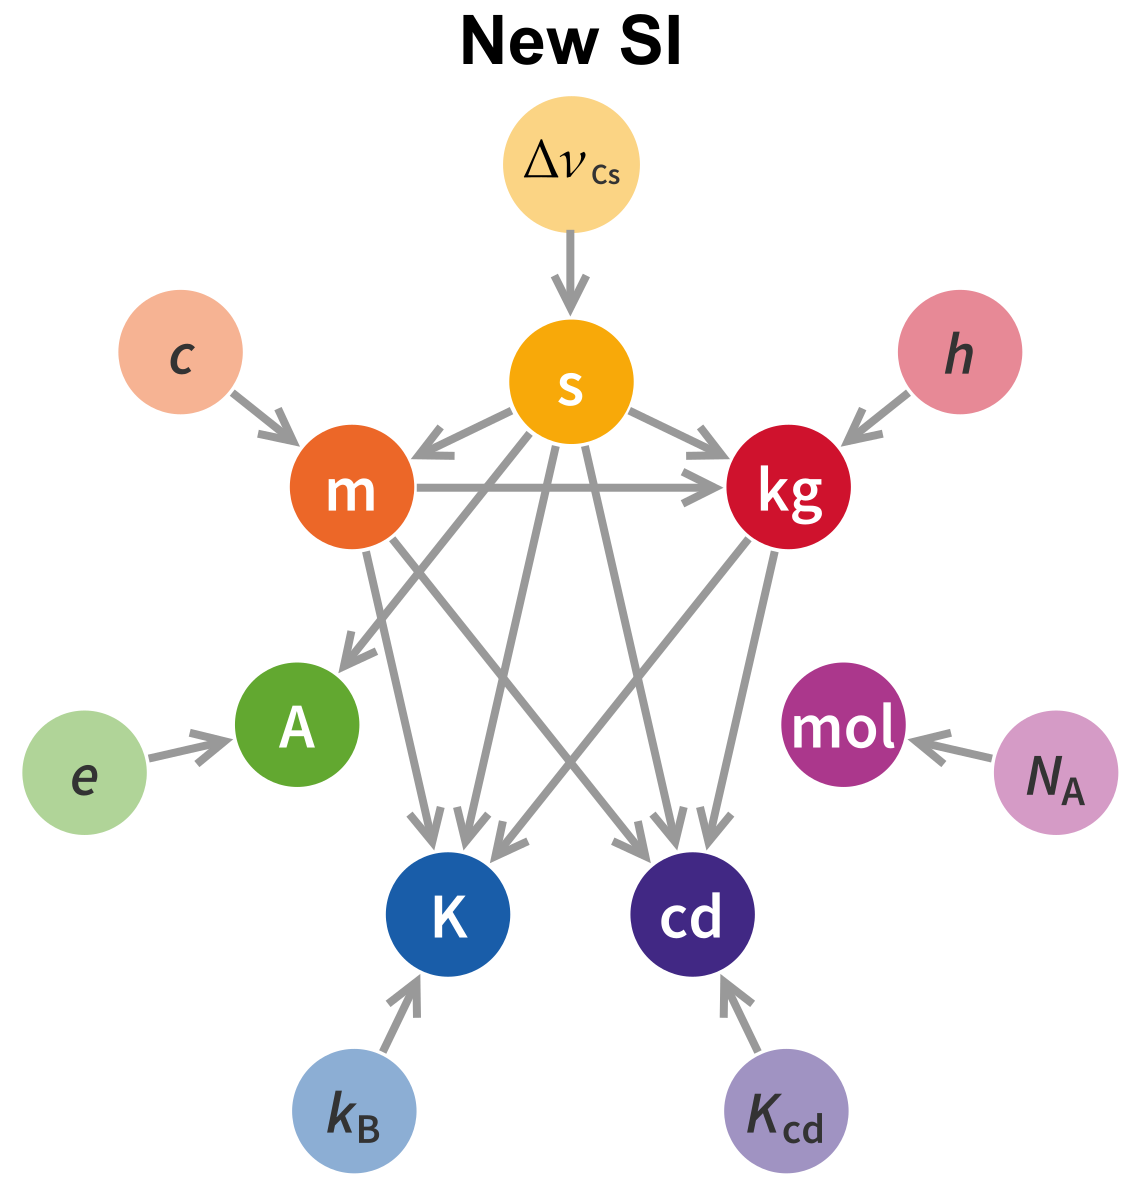
\includegraphics[height=2.5in]{images/unit_relations_SI.png}
\caption{测量问题:SI 2019 中基本量和物理常数之间的关系}
\end{figure}

在将\gls{邱奇论题}应用于\gls{形式系统}时,我们注意到上述相应的\gls{编码}和\gls{解码}箭头本身代表\textbf{形式}过程,实际上可以合并到论题本身。
然而,当我们想要比较一个受\gls{因果}支配的自然系统和一个受\gls{蕴涵}支配的\gls{形式系统}时,情况就不一样了。
\gls{编码工具},或\gls{转换器},现在本身就是\gls{物质系统};也就是说,是由\gls{因果}而不是\gls{蕴涵}所支配。
如上所述,它们(在最广泛的意义上)是\textbf{仪表}。因为这些仪表受\gls{因果}支配,它们所做的任何事情在\gls{物质}意义上都是\textbf{有效}的。
但是很明显,\gls{编码过程}的\gls{形式化}需要更多的\gls{模型};这依次又需要它们自己的\gls{编码}和\gls{解码过程},这就需要更多的\gls{模型},等等,一个无穷回归。
正是这一事实使物理学中的“\gls{测量问题}”变得如此困难。
这个潜在的无穷回归是否可以在某个有限点终止的问题是一个关于世界本质的深刻的认识论问题,与还原论这样的事物有着密切的联系。
我们当然不能在这里进入这样的问题;我们只是假设从自然世界到输入码带的一套仪表或其他\gls{转换器}是\textbf{给定的},
并且可以相对于\textbf{这些}\gls{编码}对\gls{邱奇论题}进行考察(然后,通过假设,\gls{编码}在\gls{物质}意义是有效的)。

我们的第二个观察在认识论上也很重要。它说,一个\gls{物质系统}的所有相关特征,以及它最初被\gls{编码}进去的\gls{模型}的所有相关特征(参见图式一) ,
都被表示为\textbf{输入字符串},由一台\textbf{其结构本身不\gls{编码}任何东西}的机器处理。也就是说,控制这些机器操作的规则,以及\gls{字符串处理}系统本身的整个\gls{推理结构},
与被\gls{编码}的\gls{物质系统}毫无关系。\textbf{唯一}的要求是,在输入字符串的\gls{编码}和结果输出字符串的\gls{解码}之间保持必要的交换性,如上文第1节所述。
正如我们将看到的,这就是\textbf{\gls{模拟}}的本质。

我们已经注意到,\gls{邱奇论题}相当于断言,所有的\gls{因果关系},可以表达成纯粹的\gls{语法项}。
我们现在可以更明确地阐述这个\gls{命题}: 相对于将自然系统的任何特定\gls{编码}转化为输入字符串,\gls{字符串处理}机器本身不能对\gls{物质系统}的任何方面进行\gls{编码}。
也就是说,机器的“\gls{硬件}”必须完全独立于\gls{生成}要处理的字符串的“\gls{硬件}”。 如果不能做到这一点,那么\gls{邱奇论题}就不可能是正确的。

鉴于上述,\gls{邱奇论题}断言,对所有\gls{物质过程},\gls{图灵机}构成了一类\textbf{\gls{通用模拟器}}。 这里有两个问题要问: (a)这是真的吗?(b)如果是,那意味着什么?

\section{邱奇论题在物理上是正确的吗?}

前面几节论证的结果如下。大自然为我们提供了大量的\gls{物质过程},我们称之为“有效”。
这些过程(我们假设)受\gls{因果}支配,而不像在\gls{形式系统}中那样受\gls{蕴涵}或\gls{产生规则}支配。
在这样的术语中,\gls{邱奇论题}可以表达如下:给定任何如此的过程,我们可以将有关\gls{生成}此过程的自然系统的适当\gls{命题}\gls{编码}到一个\gls{图灵机}的一组输入码带上;
而相应的输出码带可以被\gls{解码},从而完美地\textbf{\gls{模拟}}了有关的过程。同样地,\gls{邱奇论题}断言,所有关于\gls{物质过程}的“信息” ,因此所有的\gls{自然法则},
都可以用纯粹的\gls{语法项}来表达。

我们从哥德尔定理中知道,足够丰富的\gls{形式系统}总是包含一些不能从\gls{语法}上得到的推论。
更具体地说,给定任何\gls{命题}\gls{编码}方案,它将系统的\gls{命题}\gls{编码}到\gls{图灵机}的输入码带上,都将有系统的“真”的\gls{命题},它不会出现在任何输出码带上。
因此,建立这种推论为“真”的过程是\textbf{无效的};它们原则上,不能被任何\gls{图灵机},在给定的编码上\gls{模拟}。
当然,我们可以随时改变\gls{编码},但这不会改变哥德尔的结论。

因此,在\gls{形式系统}中,我们已经发现纯粹的\gls{语法编码}在某种意义上会\textbf{丢失信息}。
因此,丢失的信息必须属于原始\gls{推理结构}中一个不可规约的、不可\gls{形式化}的\textbf{\gls{语义成分}}。
通过改变\gls{编码},我们可以在一定程度上改变这个\gls{语义信息}所在的位置,但是我们不能消除它。

就其本身而言,哥德尔的这个结果与\gls{邱奇论题}的\textbf{物理}真实性无关,因为它是一个纯粹形式上的结果。
但它实际上暗示了\gls{邱奇论题}的物理源泉如何可能被证实或证伪。

正如我们在上面看到的,我们比较\gls{物质过程}和\gls{形式过程}的方式是通过建立\gls{建模关系},如上面图式一所示。
\gls{物质系统}的\gls{形式化}\gls{模型}是非常好的\gls{形式系统},其\gls{推理结构}从定义上反映了被建模的自然系统中的\gls{因果过程}。
因此,如果一个\textbf{\gls{模型}},以这种方式产生,应该属于哥德尔论证的范围,这将至少是强有力的证据,证明\gls{邱奇论题},作为一个\gls{物理命题},是虚假的。
换句话说,应该会存在这样的物理过程,它们可以有效计算非递归函数。这也意味着\gls{自然法则}不能完全用\gls{语法项}来表达。

因此,显而易见要寻找的是一个\gls{物质系统}的\gls{模型},它作为一种形式体系丰富到可以“做算术”。
不幸的是,物理学以纯物理系统的\gls{模型}而提供的形式体系,仅仅作为\gls{形式系统}来考虑,是极其贫乏的。
但是,正如我们在其他地方所争论的,这些形式体系事实上是高度非通用的,不足以描绘像有机体这样的\gls{物质系统}\cite{RosenRinpress}。
表达这种非通用性的一种方式恰恰在于它们刻画\gls{因果结构}的方式。每当这种非通用性被移除一次,一类新的(\textbf{潜在})\gls{模型}就被提出了,其中\gls{因果结构}的刻画就更加丰富至极,也更加复杂。
因为,正是\gls{因果结构}的\gls{形式化}刻画是\gls{邱奇论题}的核心,我们可能会在这些形式体系中发现许多\textbf{\gls{因果}}有效的过程,但在\textbf{数学上}是无效的。
这就意味着这些系统的行为必须包含一个不可约的\gls{语义成分},一个与系统的\textbf{复杂性}密切相关的成分。

约翰·米希尔很久以前就采取了不同的方法\cite{MyhillJ1966}。
他能够证明,模掉一些理想化的\gls{测量}和性能公差,已经有经典的\gls{模拟设备}(\gls{模拟计算机}),可以“计算”非递归函数。
这样的系统将因此已经表现出任何纯粹的\gls{语法编码}无法\gls{预测}的行为,因此也将有一个不可规约的\gls{语义内容}。

最后,我们已经提到,牛顿粒子力学,以及最近基于基本粒子的统一物理理论,本身就是一种试图用纯\gls{语法项}来表达\gls{自然法则}的尝试。
由于任何\gls{物质系统}都是由这些“无意义”(即无结构)的基本单元组成的,这些理论本质上断言,要理解任意这样系统的任何行为,用这些子单元及其相互作用来描述它就足矣。
如前所述,这就是还原论的本质。

在这些项中,熟悉的拉普拉斯精灵是一个纯粹的\gls{语法}概念: 如果他可以存在的话,就是\gls{邱奇论题}的体现。
事实上,由于我们已经指出的原因,他不可能存在(或者至少不可能作为一个由粒子构成的\gls{物质系统}存在)。
但是即使他能够存在,他也是一个非常糟糕的生物学家,例如,有机体和一般的开放系统,都在不停的传递交换它们的组成粒子。
因此,即使要找到一个有机体,更不用说及时跟踪它,他也需要用系统内不可\gls{形式化}的其他(\gls{语义})信息来补充纯粹的\gls{语法信息}。

因此,由于种种原因,我们有理由相信邱奇的\gls{命题}作为一个\gls{物理命题}是失败的。
然而,正如我们已经看到的,从\gls{物质}方面去陈述和分析\gls{邱奇论题},涉及到理论科学的一些最深刻和最基本的方面。

\section{模拟的角色}

我们已经在上面提到了\gls{图灵机}的使用,它既是对\gls{物质世界}的隐喻,也是对那个世界的有效描述。
在这两种情况下,虽然以不同的方式,我们试图从纯粹的\gls{语法形式}中得出关于\gls{物质过程}的结论。
在最后一节中,我将非常简要地考虑一个著名的例子: 冯·诺依曼的“自复制自动机”\cite{BurksA1966}\cite{ArbibMA1988}。

冯·诺依曼论证的基础是根据图灵关于通用\gls{模拟器}(计算机)的论证推断“通用构造器”的存在。
在纯形式方面,冯·诺依曼构建了一个由互通\gls{图灵机}组成的宇宙(“元胞空间”),这些机器排列成规则的几何阵列,就像多细胞生物中的细胞,或者大脑中的神经元,或者晶体中的原子。
每台机器都与数组中最近的邻居通信。按照显而易见的方式,阵列作为一个整体在时间上改变“状态”。
问题是一些子阵列(“铺嵌自动机”)能否在其补上诱导出某些有趣的行为,这些行为可以\textbf{解释}为构造、复制、增长、发展、进化等等。

同时,冯·诺依曼清楚地相信“通用构造函数”可以作为\textbf{\gls{硬件}}存在。
他设想给\gls{图灵机}配备传感器,这样它就可以“读取”蓝图,并配备效应器,这样它就可以从周围环境中提取物理组件,并按照被读取的蓝图的指示组装它们。
(在这个上下文中,“效应器”是从数字到实物的\gls{转换器},例如,“反射计” — an “inverse meter”)
这里的想法是—计算和构造都是\gls{算法过程},因此任何对一个真实(true)的东西\textbf{都}必须对另一个真实。

冯·诺依曼还认为元胞空间不仅仅是形式上的构造,实际上还包含了真实世界的构造器和它行为的\textbf{\gls{模型}}。在这一点上,他默认了\gls{邱奇论题}的最强形态。

我们已经在其他地方\cite{RosenR1985}论证,根据\gls{因果关系},从一个\textbf{形式的}通用计算机的存在导出一个\textbf{\gls{物质}的}通用构造器的任何推论都是没有根据的。
在这个论证中,我们基本上表明,没有内在的方法可以区分那些\gls{编码}了“真实世界信息”的输入字符串和那些没能\gls{编码}的输入字符串。
因此,没有办法区分可以声称\gls{模拟}“真实世界”进程的计算和没有实现这种\gls{模拟}的计算。

于是,我们也可以看到,\gls{邱奇论题}的虚假性意味着\gls{物质}过程的某些方面不能被任何给定的\gls{编码}来\gls{形式化}。
因此,存在 (a)没有\gls{物质}对应物的\gls{形式构造},反之,(b)没有形式对应物的\gls{物质构造}。因此,在这两个方面,冯·诺依曼的论点都没有实质内容,
仅仅涉及到“自动机”(或“机器”)和“构造”这两个术语常见的模棱两可。

这些考虑表明,不受限制地从\gls{形式系统}外推到\gls{物质系统}是多么危险。
危险恰恰产生于这样一个事实,即计算只涉及\textbf{\gls{模拟}},这使得在\gls{物质系统}中的\gls{因果过程}和\gls{模拟器}中的\gls{推理过程}之间可以建立不一致。
因此,我们恰恰缺乏这种外推所需的\gls{编码}和\gls{解码}的基本特征。于是,尽管\gls{形式化}\gls{模拟}具有重要的实用价值和启发性价值,
但它们的理论意义却受到严格限制,使用时必须格外谨慎。

当然,在这个简短的篇幅里,我们无法触及邱奇论题的许多其他分支。正如我们已经看到的,它的主要作用是将\gls{形式系统}中的\gls{语法}部分和非语法部分区分开来;
当\gls{形式系统}也是\gls{物质系统}的\gls{模型}时,\gls{邱奇论题}对\gls{因果关系}也做了同样的事情。事实上,这篇论文提出了一系列关于\gls{自然法则}、\gls{因果关系}、建模以及\gls{形式系统}的\gls{物质}实现的深刻问题。
它的中心特征是\gls{图灵机},将\gls{语法}或\gls{字符串处理}的本质体现在一个单一的、概念丰富的包中。即使(我相信)\gls{邱奇论题}失败了,它也是以一种最富教育意义的方式失败的。
它对\gls{物质科学},尤其是生物学的影响,还没有开始探索。

\newpage
\phantomsection
\addcontentsline{toc}{section}{参考文献}
\bibliographystyle{ieeetr}
\bibliography{biblio/article}

\newpage
\phantomsection
\addcontentsline{toc}{section}{术语列表}
\printindex
\printglossaries

\newpage
\appendix
\section{术语共现图}

\begin{figure}[ht]
\centering
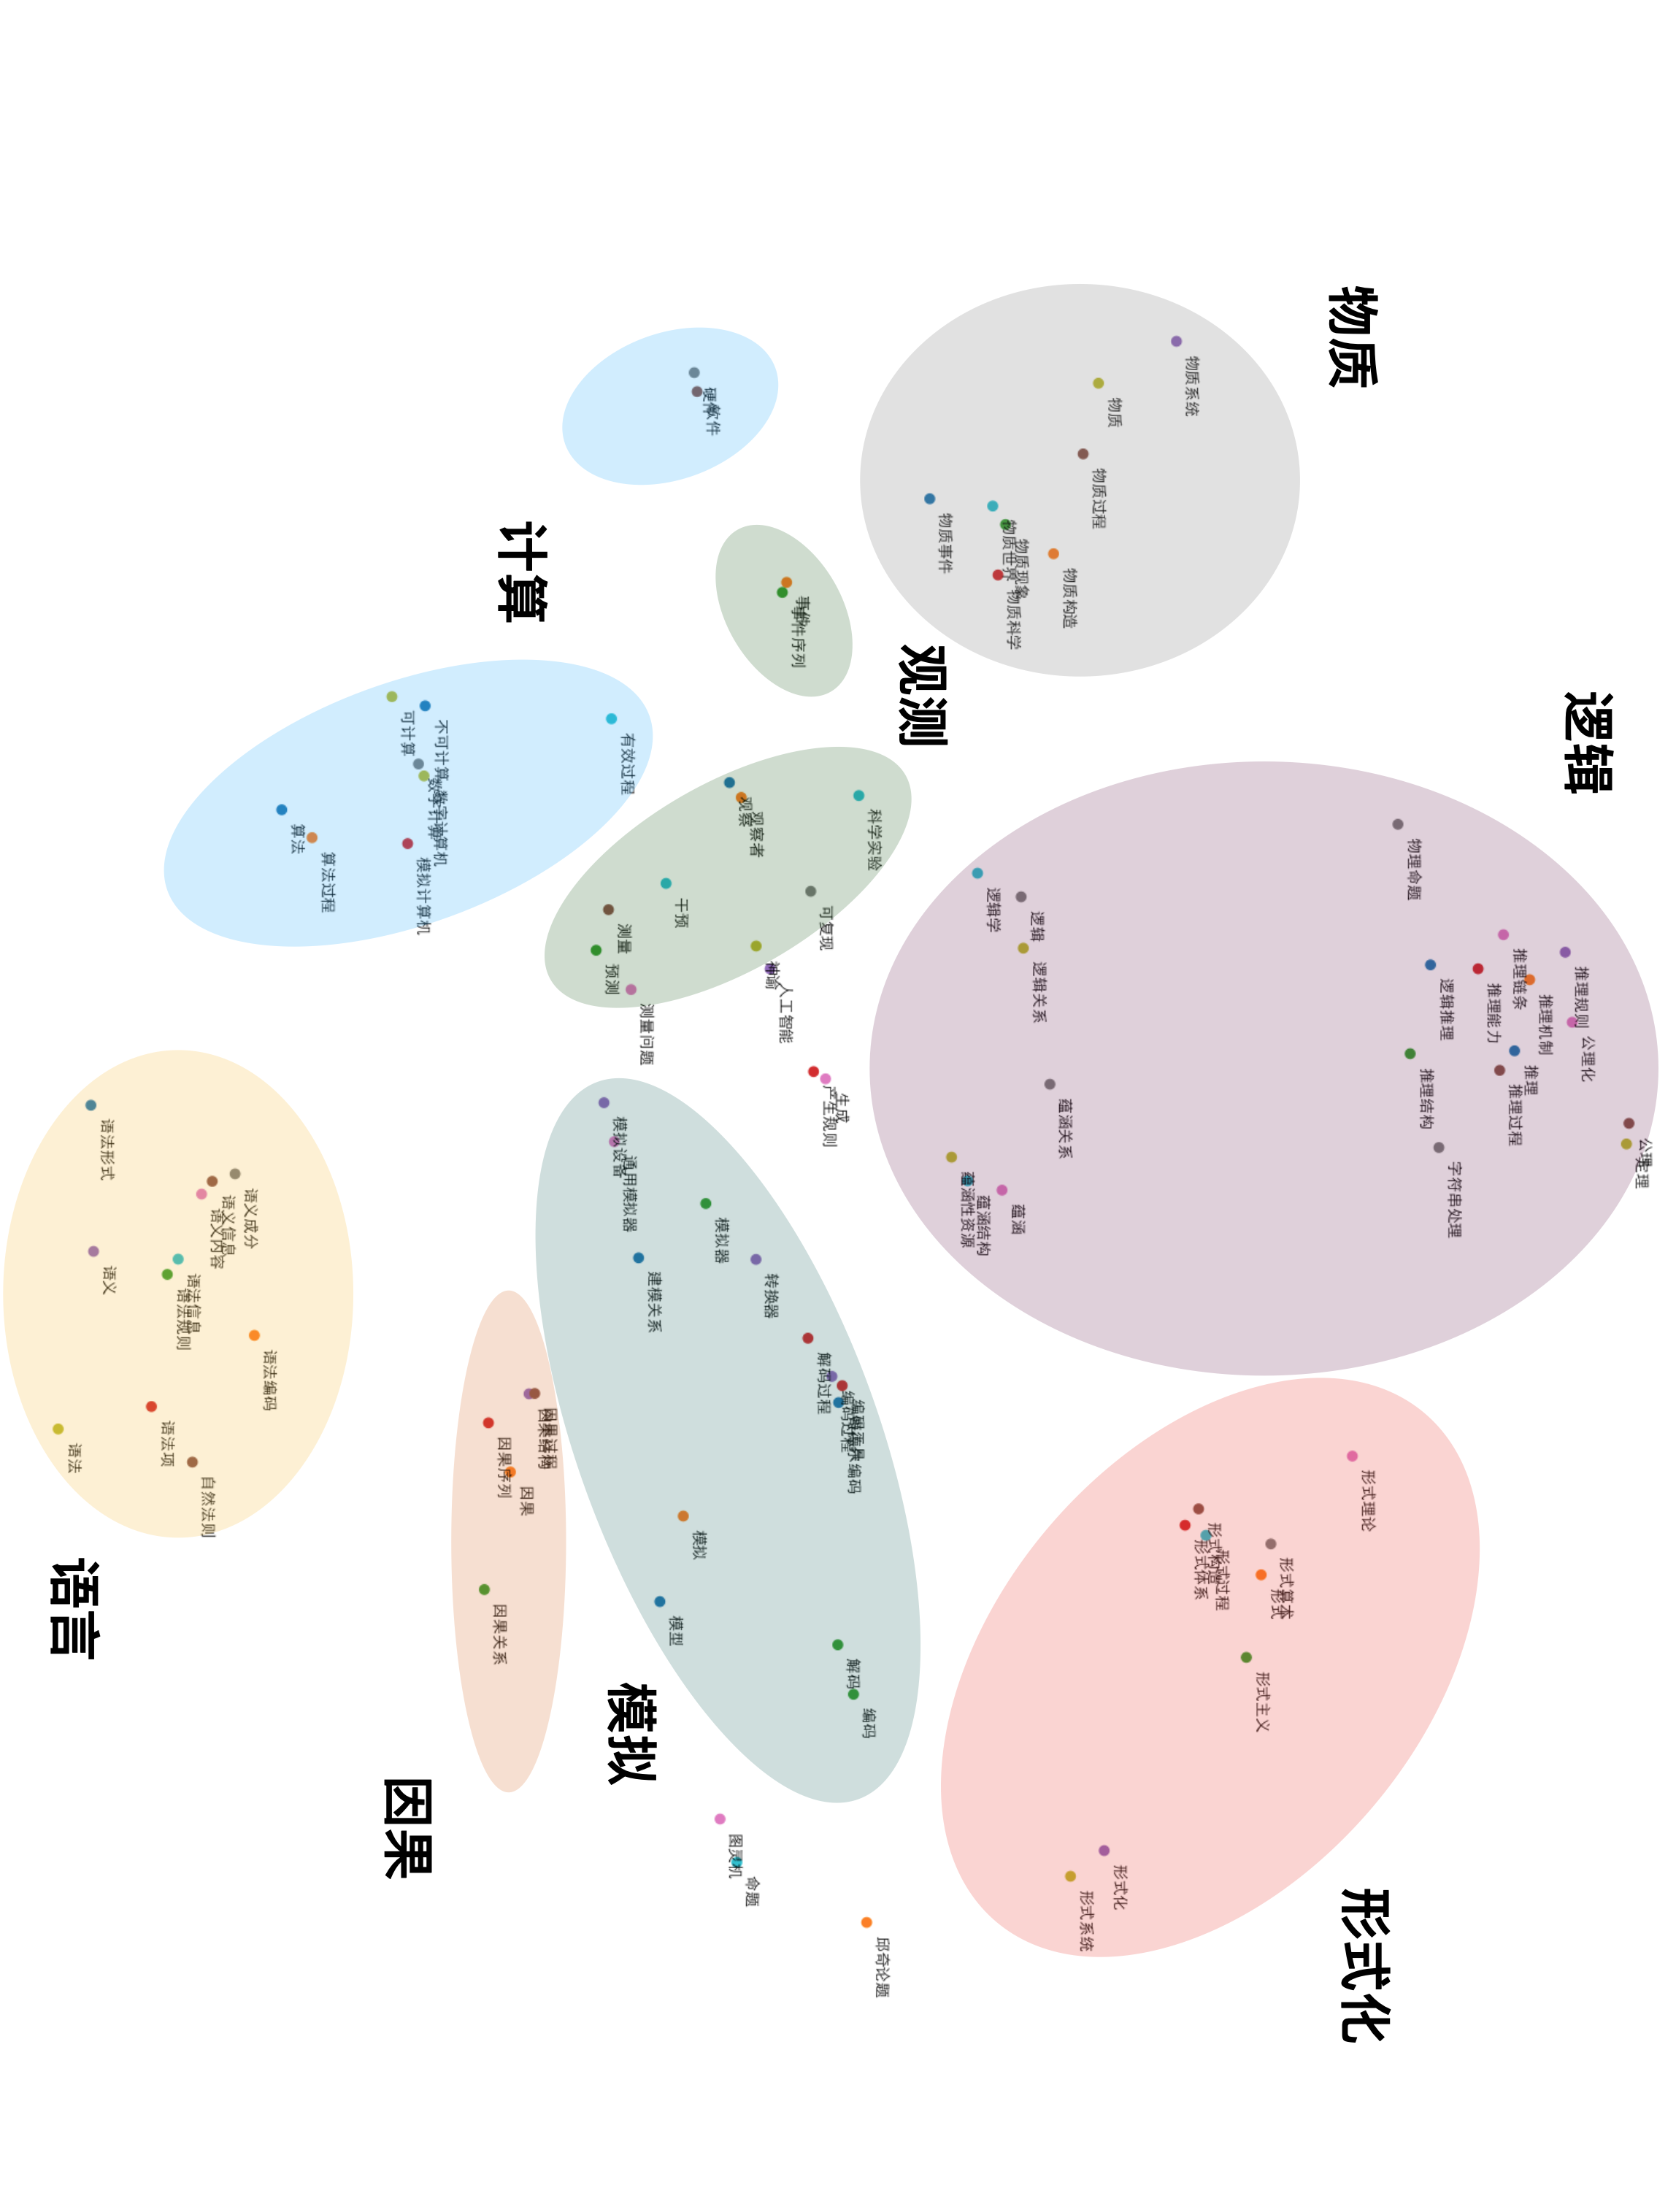
\includegraphics[height=7in]{images/concepts.png}
\caption{术语共现图}
\end{figure}

\newpage
\section{译后小记}

大约八年前,在参与集智的周末研读活动的时候,我收集了一批关于计算和物理的交叉领域的文章。
那个时候,就发现了 Robert Rosen 的这篇《有效过程与自然法则》写的很特别,非常富有洞见。
但因为有些意思相对曲折,读起来也有些困难,于是就产生了通过翻译来学习这篇文章的想法。

说这篇文章特别,是因为计算机科学从 1930 年代开始,已然长成参天大树,学科的各个分支枝繁叶茂,发表的文章不计其数,
但少有深入到学科源头去探讨一番的文章。也正因为如此,这篇富有哲理的文章也常读常新。

举例来说,在文章的引言,作者把 McCulloch 和 Pitts 的工作与 G{\"o}del 的发现并列,这里面的意味颇值得思考。
罗伯特·罗森写作的当时是 AI 的寒冬,为什么会这么写呢? 从文章内容冒昧揣测,他作为生物学家的特有视角发挥了作用。
但由于时代的局限,罗森并没有把 McCulloch 等人工作的重要做充分的展开。
今天,神经网络、深度学习获得了极大的发展,大家都意识到了神经网络在工程实践方面的重要,但如何从理论上申明罗森的视角的有趣之处呢?

\begin{figure}[ht]
\centering

\includegraphics[height=2.5in]{images/landscape.png}
\caption{向下去探索}
\end{figure}

和罗伯特·罗森做的一样,让我们试着回到源头。在源头,“学习”是一个可以和“计算”并列的理论题目。
从 1967 年 E. Mark Gold 的经典论文 Language identification in the limit 起,这一分支开始发展, 后经 Leslie Valiant 的 PAC 理论开始成型。
但我想提及一篇少为人知的重要论文, 1996 年 R. Lathrop 在 ICML 上发表了 On the Learnability of the Uncomputable ,
论文表明通过分析程序运行的时空行为,在概率意义上停机问题可学习。 论文在可计算性和可学习性之间给我们找到了一块落脚石,
同时论文的分析方法和算法信息论(AIT)里 Chaitin 常数 $\Omega$ 的渐进可计算性似乎有更进一步的联系。
我们或许可以沿着可学习性这条小径重新思考罗伯特·罗森的所思所想。

从去年起,我利用零零散散的时间,开始了这个翻译工作。在朋友们的帮助之下,今天终于把本文翻译完毕。在此,对集智同学们多年的支持和杨文波同学的校读一并表示感谢。

\hfill \hfill 2021 年 5 月

\hfill \hfill 明理

\end{document}


